\documentclass{ximera}
%% You can put user macros here
%% However, you cannot make new environments

\listfiles

\graphicspath{{./}{firstExample/}{secondExample/}}

\usepackage{tikz}
\usepackage{tkz-euclide}
\usepackage{tikz-3dplot}
\usepackage{tikz-cd}
\usetikzlibrary{shapes.geometric}
\usetikzlibrary{arrows}
\usetkzobj{all}
\pgfplotsset{compat=1.13} % prevents compile error.

%\renewcommand{\vec}[1]{\mathbf{#1}}
\renewcommand{\vec}{\mathbf}
\newcommand{\RR}{\mathbb{R}}
\newcommand{\dfn}{\textit}
\newcommand{\dotp}{\cdot}
\newcommand{\id}{\text{id}}
\newcommand\norm[1]{\left\lVert#1\right\rVert}
 
\newtheorem{general}{Generalization}
\newtheorem{initprob}{Exploration Problem}

\tikzstyle geometryDiagrams=[ultra thick,color=blue!50!black]

%\DefineVerbatimEnvironment{octave}{Verbatim}{numbers=left,frame=lines,label=Octave,labelposition=topline}



\usepackage{mathtools}


\title{Where was Eye?} \license{CC BY-NC-SA 4.0}

\begin{document}

\begin{abstract}
We determine the location of the camera based on a photograph it took.
\end{abstract}
\maketitle

\section*{Where was Eye?}

\begin{image}
         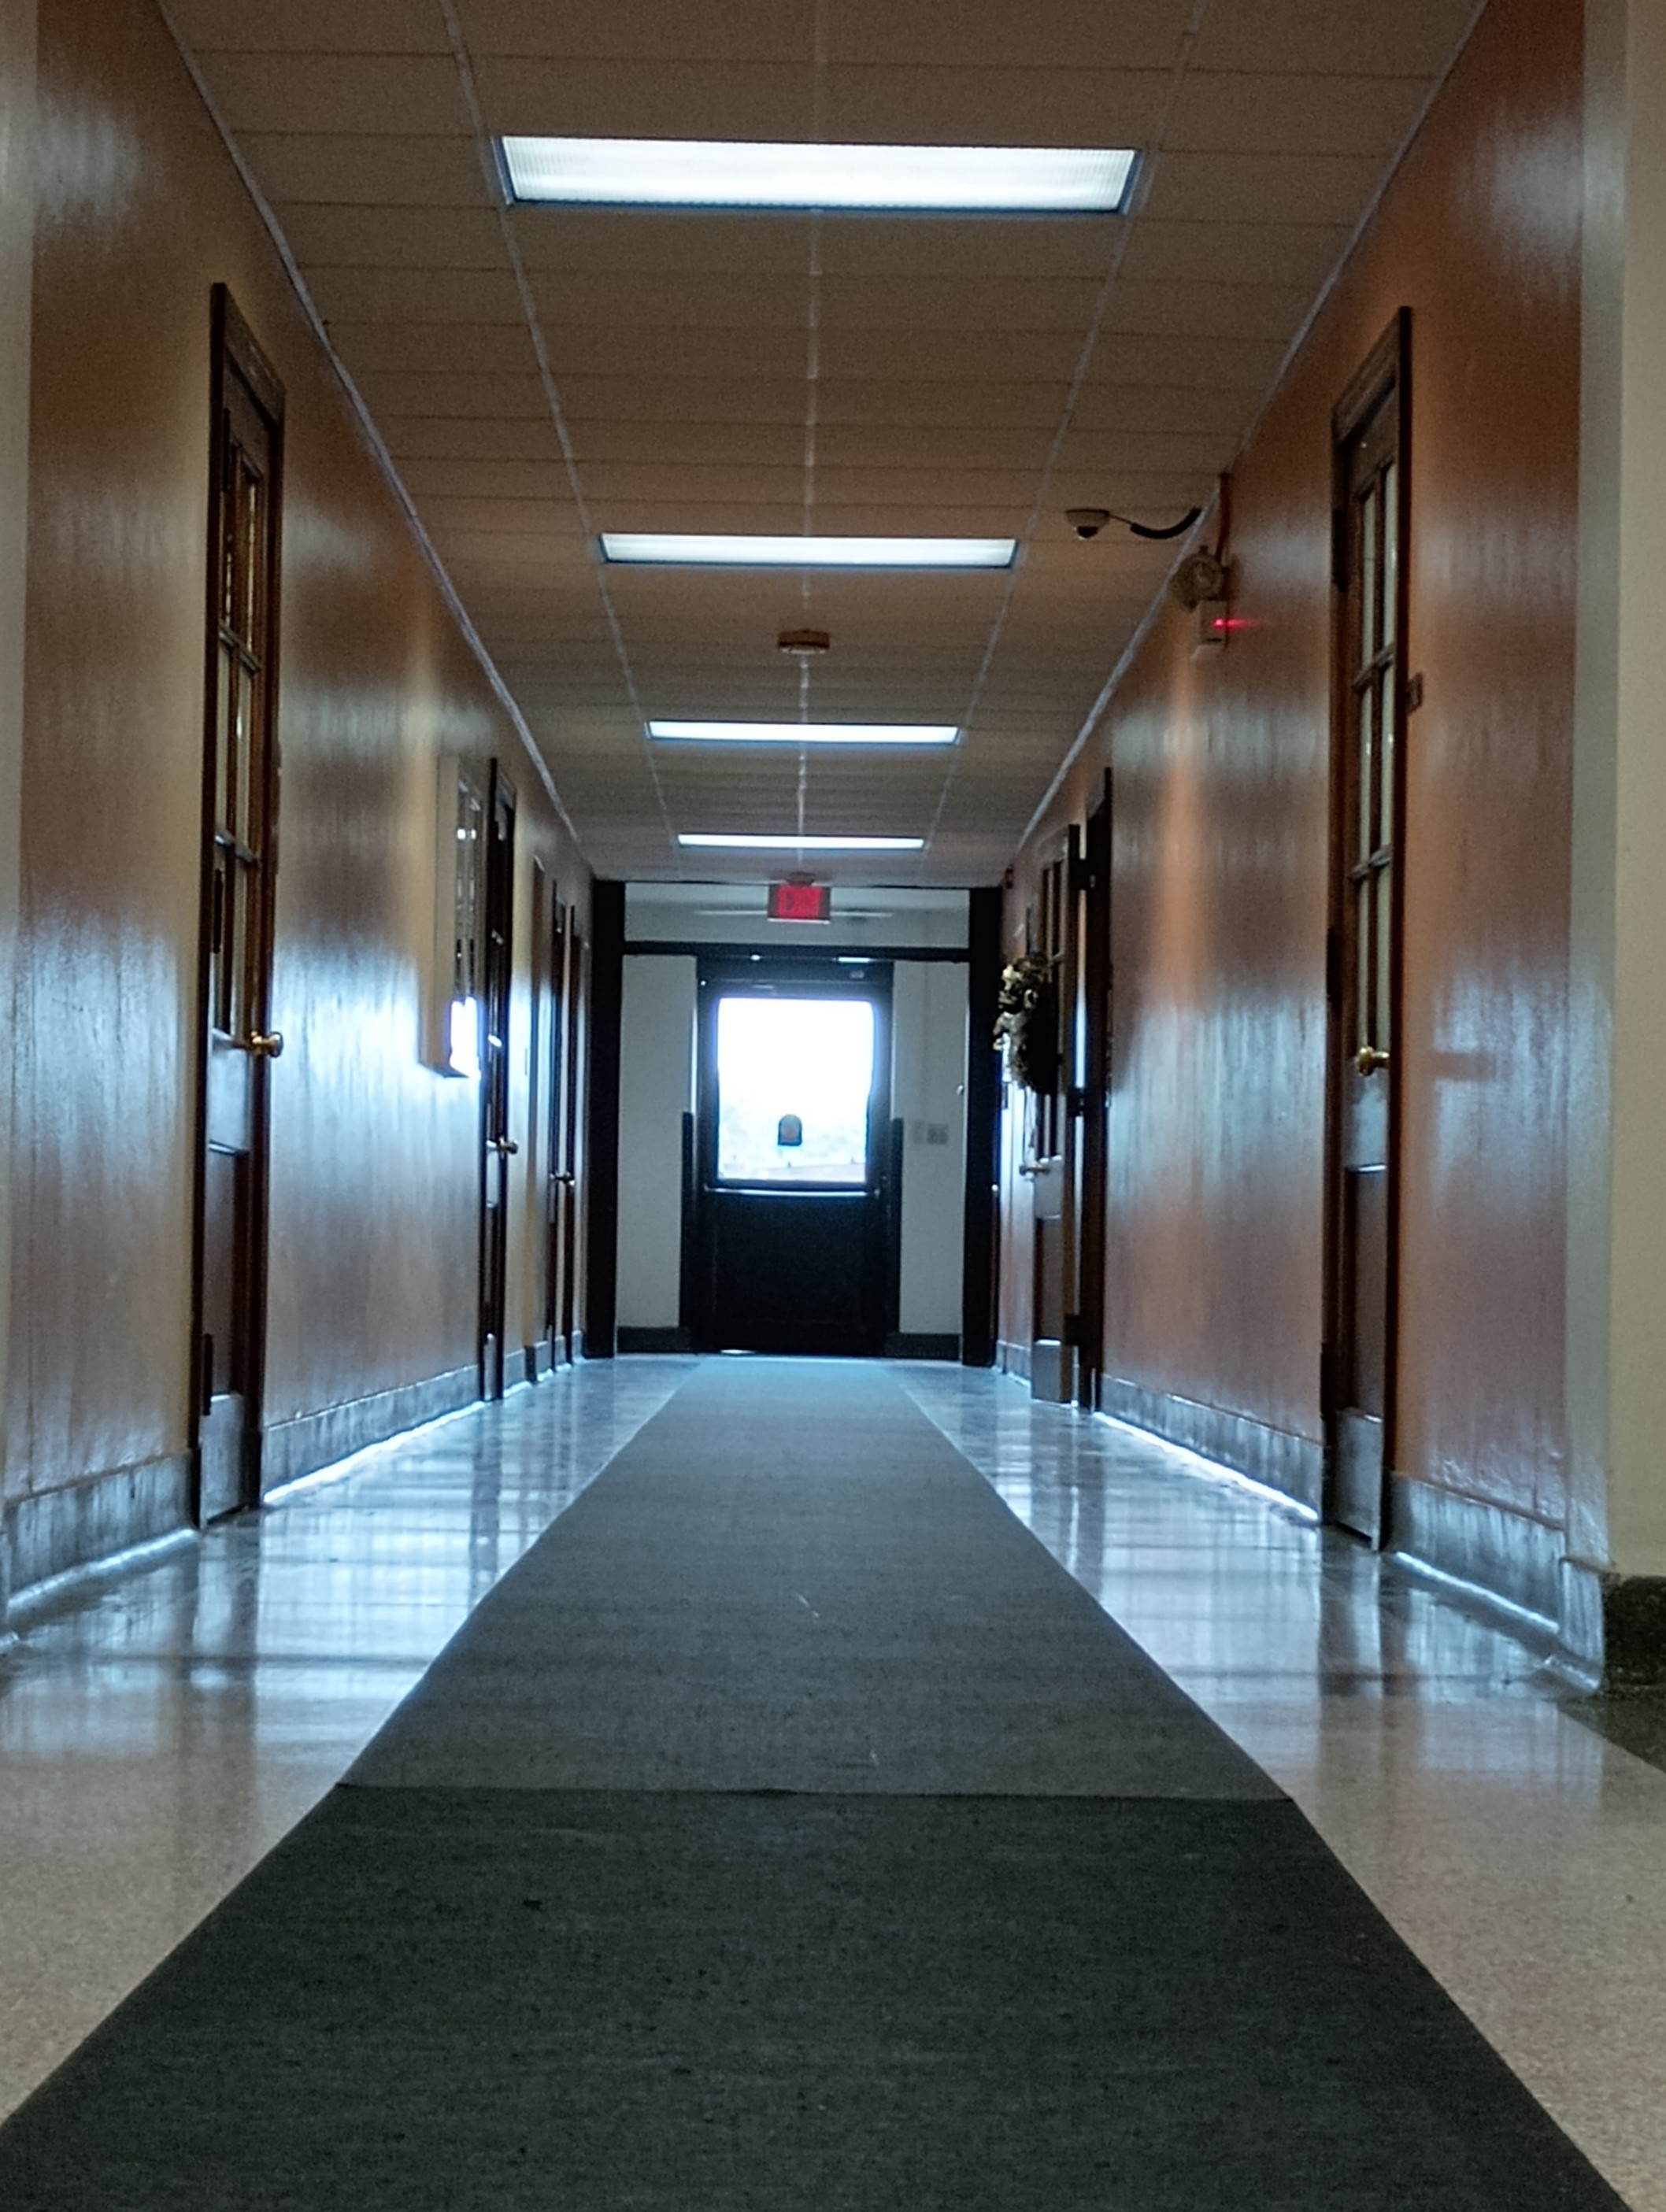
\includegraphics{hall1.jpg}
\end{image}

\begin{image}
         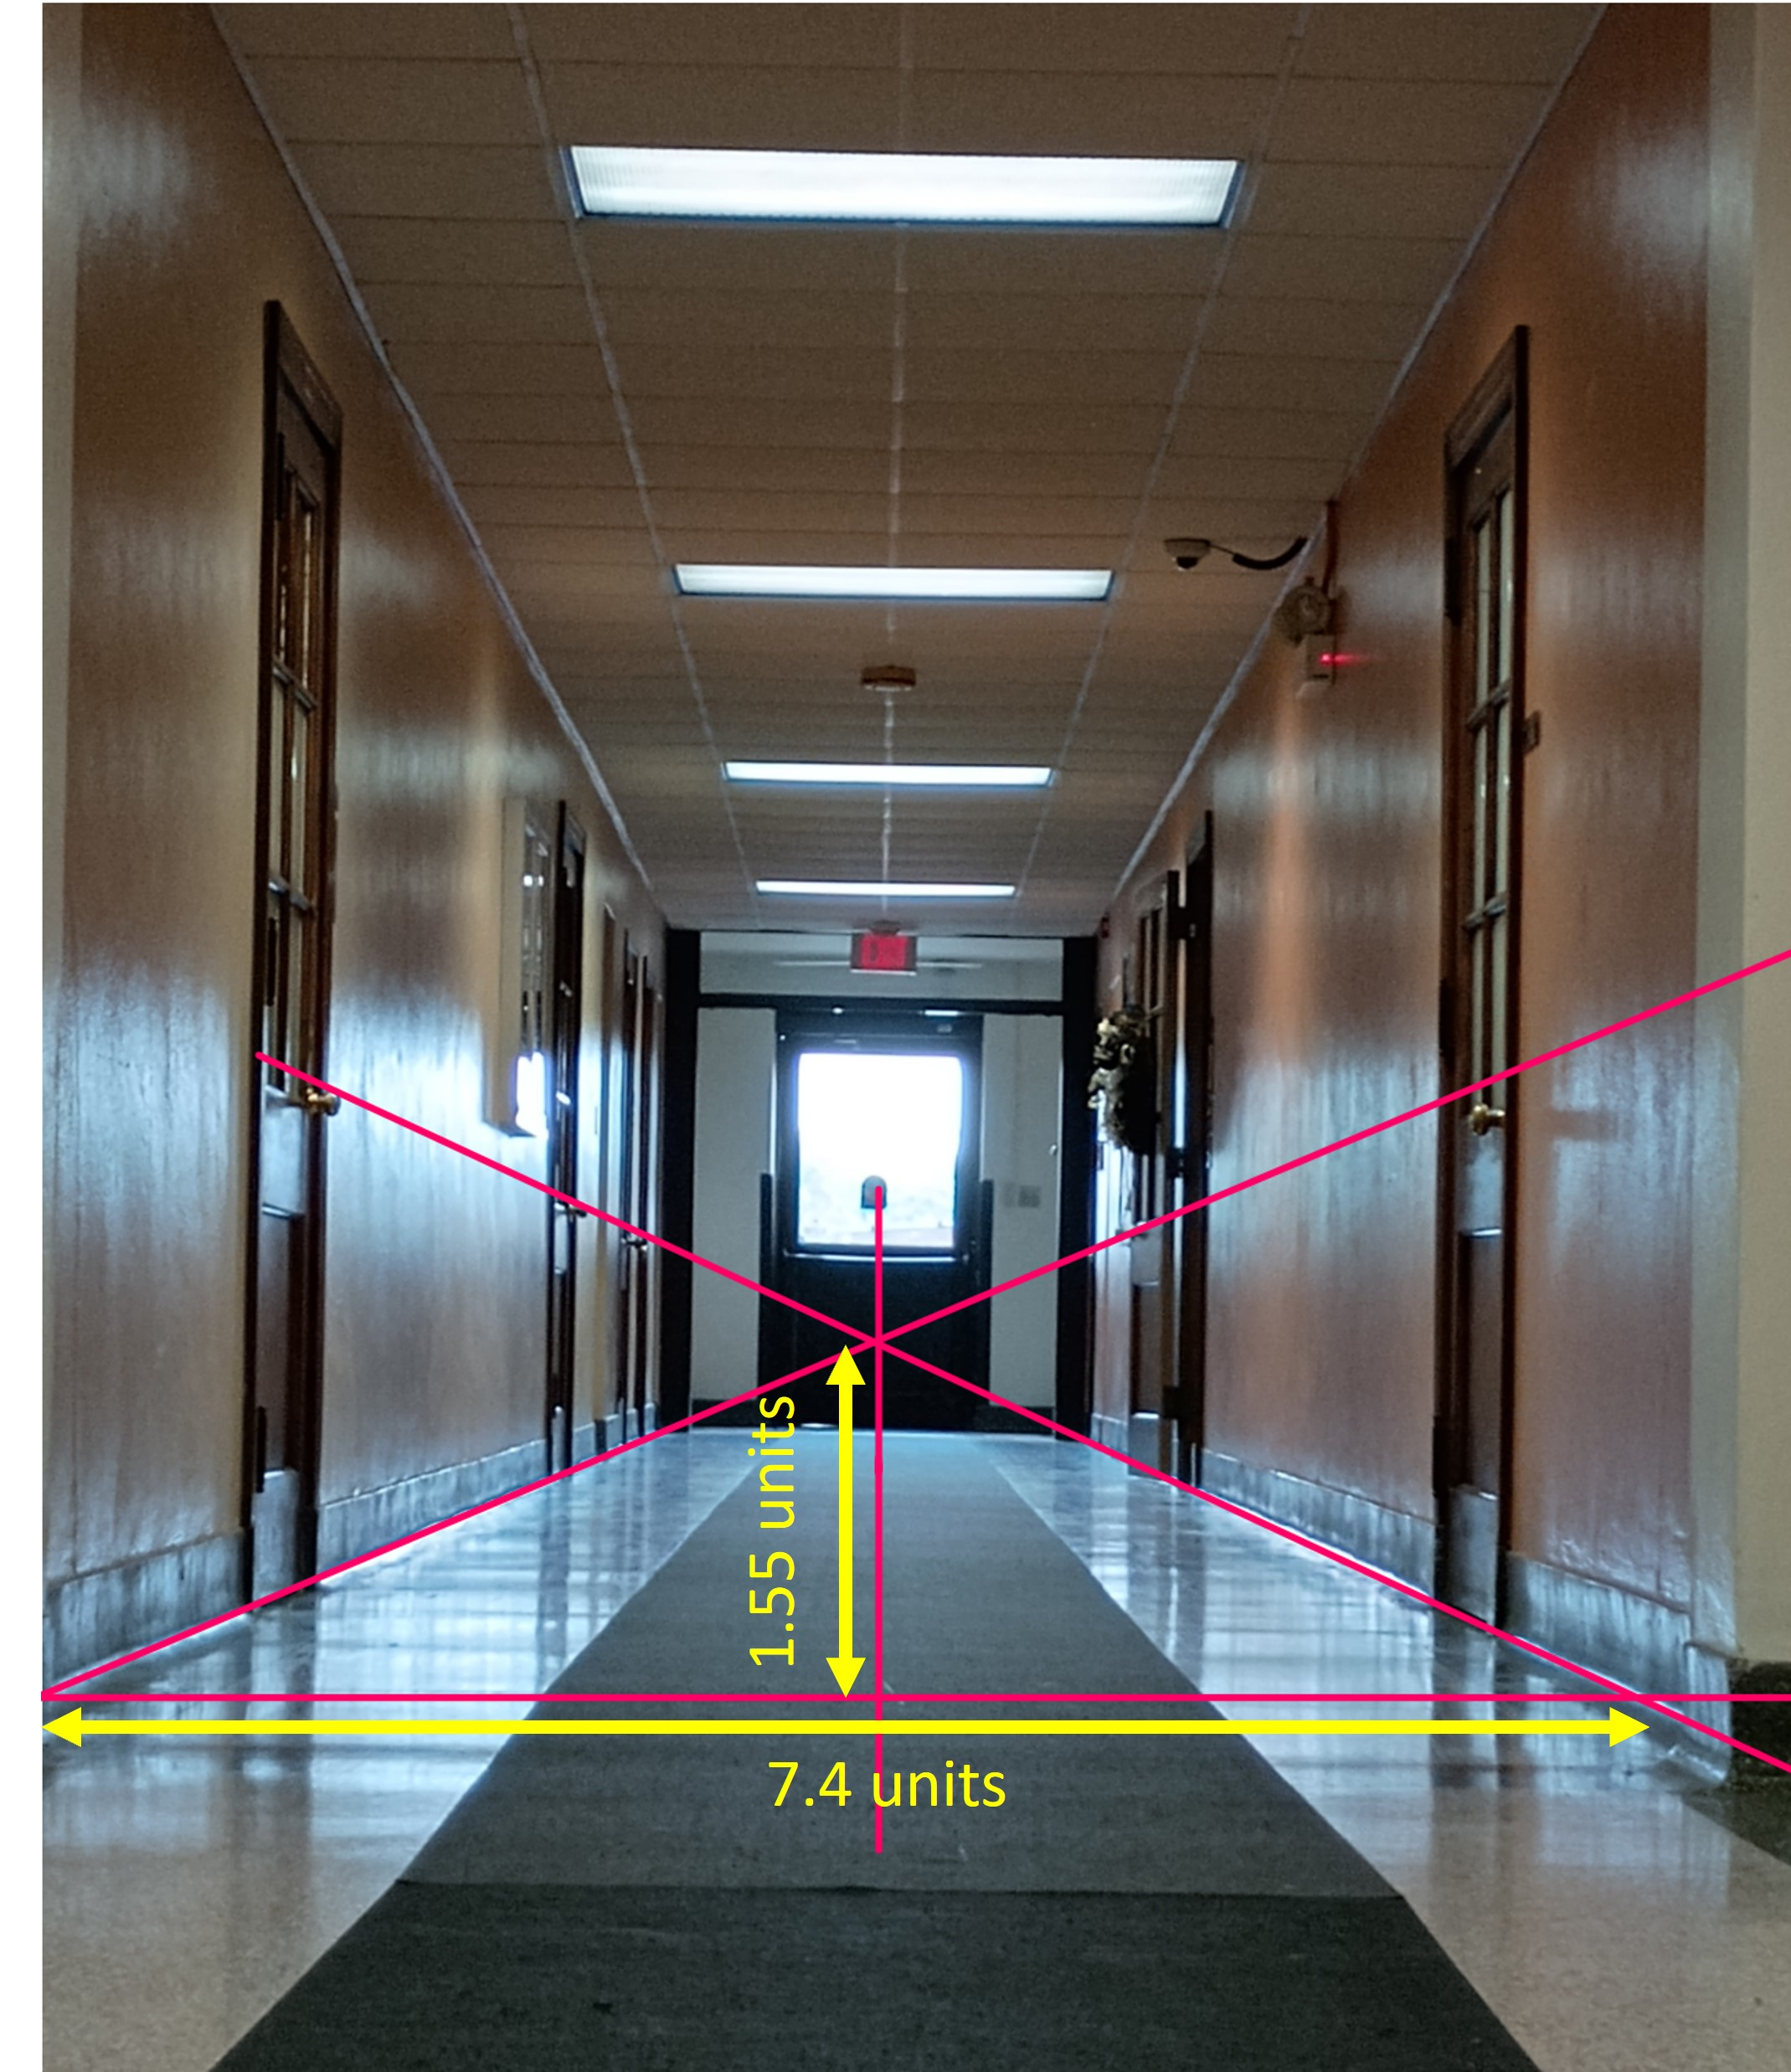
\includegraphics{hall2.jpg}
\end{image}

\begin{onlineOnly}
\begin{center}
\geogebra{bgwstwyy}{950}{500}
\end{center}
\end{onlineOnly}

\begin{onlineOnly}
\begin{center}
\geogebra{nakhdsae}{950}{500}
\end{center}
\end{onlineOnly}

\begin{onlineOnly}
\begin{center} 
\desmos{vhywzefinc}{800}{600} 
\end{center}
\end{onlineOnly}






\end{document}